% ============================================================
%  Explanation-Supervised Attention CNN — Final Course Report
%  CSCD 618 / DSCD 604 — University of Ghana
%  Format: CVPR / ECCV / ICCV style (two-column, 10pt, 5-7 pp.)
%
%  Compile:
%    pdflatex DL_Final_Report_Conference
%    bibtex   DL_Final_Report_Conference
%    pdflatex DL_Final_Report_Conference
%    pdflatex DL_Final_Report_Conference
% ============================================================
\documentclass[10pt,twocolumn,letterpaper]{article}

% ── Geometry (CVPR 2024 margins) ─────────────────────────────
\usepackage[letterpaper,
            top=2.54cm, bottom=3.81cm,
            left=2.22cm, right=2.22cm,
            columnsep=0.95cm]{geometry}

% ── Fonts & encoding ─────────────────────────────────────────
\usepackage[T1]{fontenc}
\usepackage[utf8]{inputenc}
\usepackage{times}
\usepackage{microtype}

% ── Math & symbols ───────────────────────────────────────────
\usepackage{amsmath,amssymb}
\usepackage{pifont}

% ── Graphics & tables ────────────────────────────────────────
\usepackage{graphicx}
\usepackage{booktabs}
\usepackage{multirow}
\usepackage{array}
\usepackage{subcaption}
\usepackage{float}

% ── Colours & hyperlinks ─────────────────────────────────────
\usepackage{xcolor}
\usepackage[colorlinks=true,
            linkcolor=blue!70!black,
            citecolor=blue!70!black,
            urlcolor=blue!70!black]{hyperref}

% ── Bibliography ─────────────────────────────────────────────
\usepackage{natbib}

% ── TikZ ─────────────────────────────────────────────────────
\usepackage{tikz}
\usetikzlibrary{shapes.geometric,arrows.meta,positioning,calc,fit,backgrounds}

% ── Lists & spacing ──────────────────────────────────────────
\usepackage{enumitem}
\usepackage{parskip}
\setlength{\parskip}{2pt}
\setlength{\parindent}{0pt}

% ── Section formatting (CVPR-like) ───────────────────────────
\usepackage{titlesec}
\titleformat{\section}{\normalsize\bfseries\centering}{}{0em}{\thesection.\quad}
\titleformat{\subsection}{\small\bfseries}{}{0em}{\thesubsection.\quad}
\titleformat{\subsubsection}{\small\itshape}{}{0em}{\thesubsubsection.\quad}
\titlespacing{\section}{0pt}{6pt}{2pt}
\titlespacing{\subsection}{0pt}{4pt}{1pt}
\titlespacing{\subsubsection}{0pt}{2pt}{1pt}

% ── Caption styling ──────────────────────────────────────────
\usepackage[font=small,labelfont=bf,skip=3pt]{caption}

% ── Custom column ─────────────────────────────────────────────
\newcolumntype{C}[1]{>{\centering\arraybackslash}p{#1}}

% ── Dagger for footnote marks (avoid conflict with LaTeX built-in) ──
\newcommand{\dagmark}{$^{\dagger}$}

% ─────────────────────────────────────────────────────────────
\begin{document}

% ── Title block ──────────────────────────────────────────────
\twocolumn[{%
\begin{center}
  {\large\bfseries
   Explanation-Supervised Attention for Multi-Label Thoracic\\[2pt]
   Disease Classification: A Proof-of-Concept Study}\\[8pt]
  {\normalsize
   Israel Agyekum \quad Joel Dadi-Klutse \quad Eric Okyere}\\[3pt]
  {\small University of Ghana --- Department of Computer Science}\\
  {\small CSCD 618 / DSCD 604 --- Algorithmic Track \quad June 2026}\\[8pt]
\end{center}
\noindent\rule{\linewidth}{0.4pt}
\begin{center}{\small\bfseries Abstract}\end{center}
{\small
Post-hoc saliency methods such as Grad-CAM explain CNN decisions after training and
provide no guarantee of spatial faithfulness. We propose an \emph{explanation-supervised
attention CNN} that promotes the spatial attention map from an implicit intermediate
feature to a first-class trainable output, supervised directly by clinician-annotated
bounding-box masks. A label-correlation-aware loss further regularises predictions
against empirical disease co-occurrence statistics.
We conduct a proof-of-concept study on a \emph{class-balanced $\approx$5,000-image
subset} of NIH ChestX-ray14 (112,120 images, 14 pathologies), necessitated by
academic compute constraints; full-dataset replication is the primary extension.
Across seven model configurations (three backbone baselines, two full variants, two
ablations), supervised attention achieves mean IoU of 0.299 vs.\ 0.222 for Grad-CAM
(+34.7\% relative) and pointing-game accuracy 0.506 vs.\ 0.481 on ResNet50, at a
classification AUC cost of $-$9.9 pp (0.760 vs.\ 0.843). Ablations confirm that the
attention alignment loss drives localisation gains, while the correlation regulariser
partially recovers classification AUC. DeLong's test confirms all AUC differences are
statistically significant.
}\\[3pt]
\noindent\rule{\linewidth}{0.4pt}
\vspace{6pt}
}]

% ─────────────────────────────────────────────────────────────
\section{Introduction}
% ─────────────────────────────────────────────────────────────

Chest radiography (CXR) is the front-line thoracic imaging modality worldwide, yet
reliable interpretation requires radiological expertise that is unevenly distributed
globally --- a gap especially acute in sub-Saharan Africa where diagnostic delay is a
significant barrier to care. Deep convolutional neural networks (CNNs) have matched or
exceeded radiologist accuracy on NIH ChestX-ray14 \citep{wang2017chestxray}, yet
function as opaque black boxes, limiting clinical trust.

Standard practice applies Grad-CAM post-hoc as a spatial explanation. Critically,
post-hoc maps are not part of the training objective and need not faithfully localise
disease foci \citep{attrinet2023}. We instead promote explanations from afterthought to
objective: a spatial attention module $\mathbf{A}_s$ is a first-class supervised
output, aligned with clinician bounding boxes via an attention alignment loss
$\mathcal{L}_{\text{attn}}$ during training. A complementary label-correlation loss
$\mathcal{L}_{\text{corr}}$ encodes clinical comorbidity structure with no extra
parameters at inference.

\textbf{Research questions.}
\textbf{RQ1:} Does explanation supervision improve localisation faithfulness (IoU,
pointing-game accuracy) over post-hoc Grad-CAM while keeping AUC competitive?
\textbf{RQ2:} What are the individual contributions of $\mathcal{L}_{\text{attn}}$
and $\mathcal{L}_{\text{corr}}$?
\textbf{RQ3:} How does backbone choice interact with attention supervision?

\textbf{Contributions.}
(1) A CBAM-style supervised spatial attention module whose map is aligned with
bounding-box masks via a composite loss (Dice + MSE on annotated images; L1 sparsity
on unannotated images), with zero additional inference cost over a standard classifier.
(2) A lightweight label-correlation regulariser requiring no architectural change.
(3) A controlled evaluation of seven configurations across both classification and
localisation metrics, with DeLong significance testing and honest reporting of
proof-of-concept scope.

% ─────────────────────────────────────────────────────────────
\section{Related Work}
% ─────────────────────────────────────────────────────────────

\noindent\textbf{Multi-label CXR classification.}
\citet{wang2017chestxray} introduced ChestX-ray14 alongside CNN baselines achieving
macro AUC of 0.745. \citet{chexnet2017} trained DenseNet-121 on the full 112K corpus
to achieve 0.841 macro AUC. \citet{holste2022} rigorously re-evaluated the benchmark
under long-tailed class distributions, exposing biases in standard training recipes;
we adopt their balanced evaluation protocol. \citet{asl2021} proposed the Asymmetric
Loss (ASL), achieving SOTA on multiple multi-label benchmarks; our classification
objective adopts ASL-inspired focal weighting.

\noindent\textbf{Post-hoc explanation and inherent interpretability.}
Grad-CAM \citep{wang2017chestxray} and its variants compute class-specific heat maps
from a frozen trained model and are not guaranteed to align with annotated lesion
regions. \citet{attrinet2023} demonstrated this directly, showing standard classifiers
frequently fail to localise disease foci, and proposed Attri-Net --- an inherently
interpretable classifier using class-specific counterfactuals --- as an alternative.

\noindent\textbf{Right-for-the-right-reasons (RRR) training.}
\citet{rao2023} systematically evaluated RRR losses, finding that the attribution
method used to compute guidance significantly affects both classification and
explanation quality. \citet{lanfredi2023} supervised CXR classifiers with radiologist
eye-tracking annotations, showing that even noisy localisation signals measurably
improve faithfulness. Our work extends this to bounding-box alignment as a scalable
weak supervision signal.

\noindent\textbf{Label dependency modelling.}
\citet{hydravit2024} proposed a multi-branch transformer (HydraViT) for CXR that
handles co-occurrence at the architecture level. We provide a complementary,
loss-level approach that requires no architectural change.

% ─────────────────────────────────────────────────────────────
\section{Method}
% ─────────────────────────────────────────────────────────────

\subsection{Dataset and Splits}

NIH ChestX-ray14 \citep{wang2017chestxray} contains 112,120 frontal CXRs from 30,805
patients with 14 thoracic finding labels per image. A clinician-annotated subset
provides 984 bounding boxes across 880 images for 8 findings: Atelectasis,
Cardiomegaly, Effusion, Infiltration, Mass, Nodule, Pneumonia, and Pneumothorax.

Splits are performed at the \emph{patient level} (80/10/10, seed 42) with a verified
zero-overlap assertion, yielding 7,438 / 930 / 930 patients. \emph{Due to free-tier
Kaggle GPU constraints, we train on a class-balanced $\approx$5,000-image subset
sampled via stratified sampling. Validation and test sets retain all images in their
patient partitions for unbiased evaluation. All quantitative claims are scoped to this
subset; full-dataset replication is deferred to future work.}

\begin{figure}[t]
  \centering
  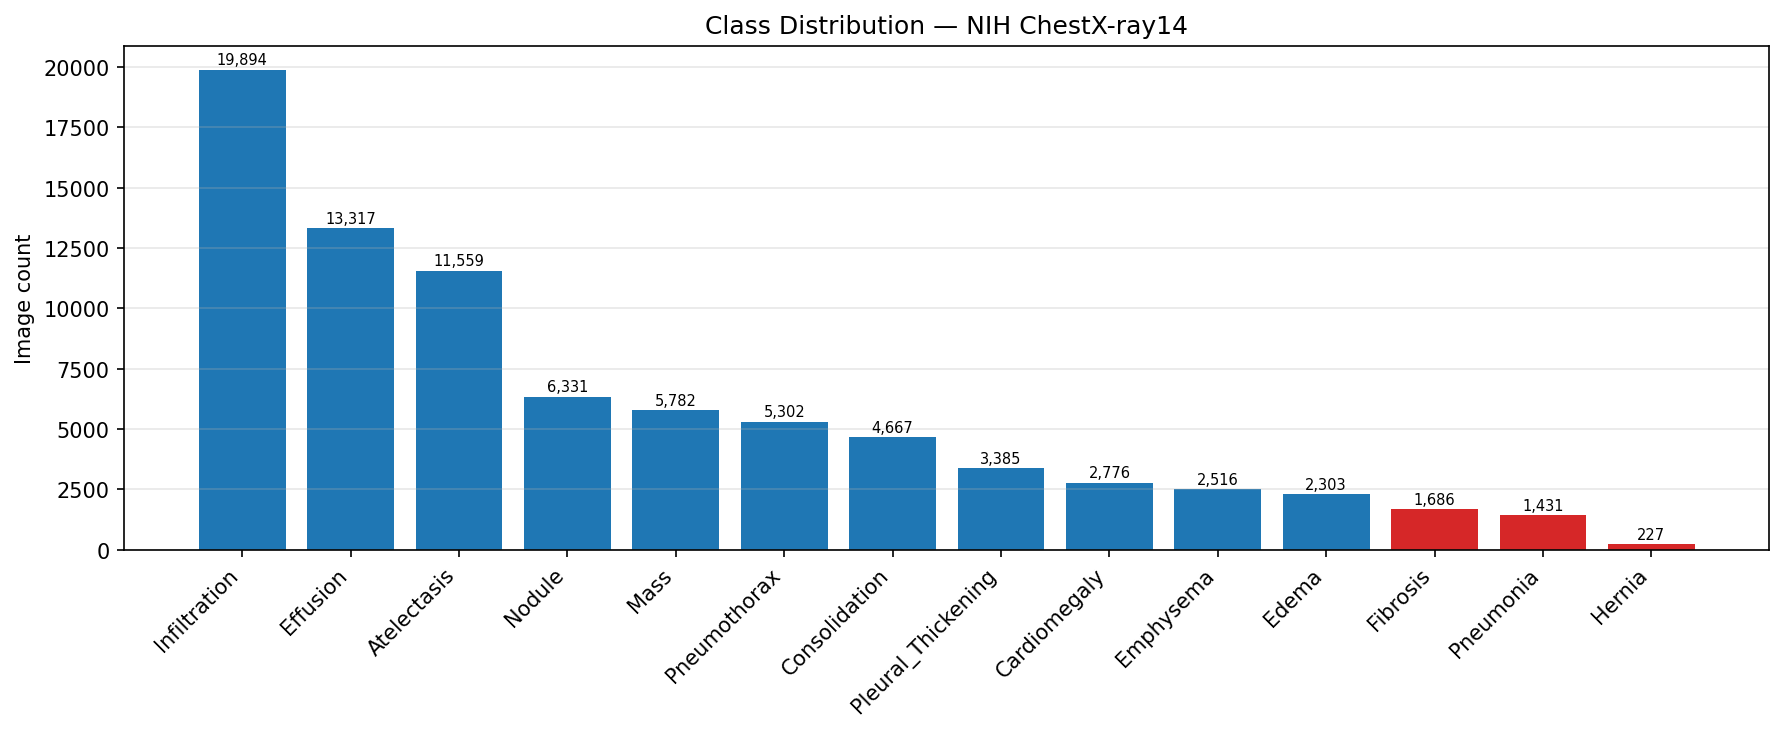
\includegraphics[width=\columnwidth]{figures/class_distribution.png}
  \caption{Per-class label frequency (training set). Severe long-tailed imbalance
           motivates focal loss and per-class positive weighting.}
  \label{fig:class_dist}
\end{figure}

Images are resized to $224\times224$ and normalised with ImageNet statistics.
Training augmentation: random horizontal flip ($p=0.5$), rotation ($\pm10^\circ$),
brightness/contrast jitter ($\pm10\%$), Gaussian blur ($p=0.1$).

\subsection{Architecture}

The pipeline (Figure~\ref{fig:arch}) has four stages: CNN backbone $\to$ optional
CBAM channel attention $\to$ supervised spatial attention $\to$ GAP + linear head.

\begin{figure}[t]
\centering
\resizebox{\columnwidth}{!}{%
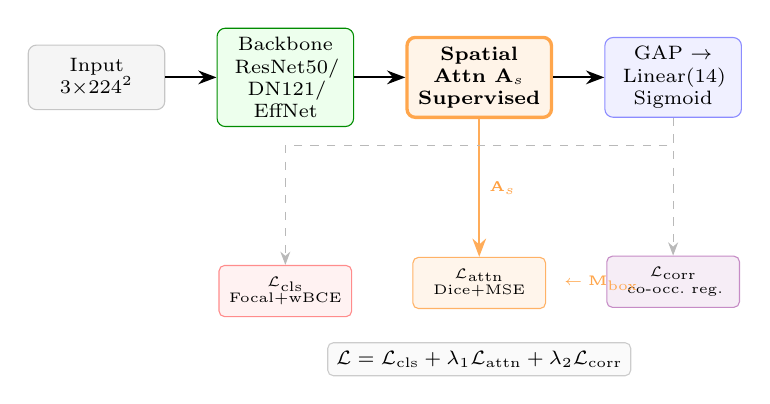
\begin{tikzpicture}[
  fwd/.style={rectangle,rounded corners=3pt,minimum width=1.55cm,minimum height=0.82cm,
              text width=1.50cm,align=center,draw=black!35,font=\scriptsize},
  bbone/.style={fwd,fill=green!7,draw=green!55!black},
  sattn/.style={rectangle,rounded corners=3pt,minimum width=1.65cm,minimum height=0.98cm,
                text width=1.60cm,align=center,draw=orange!70,line width=1.2pt,
                fill=orange!9,font=\scriptsize\bfseries},
  cls/.style={fwd,fill=blue!6,draw=blue!45},
  lbox/.style={rectangle,rounded corners=2pt,minimum width=1.55cm,minimum height=0.65cm,
               text width=1.45cm,align=center,draw=red!45,fill=red!5,font=\tiny},
  labox/.style={lbox,fill=orange!8,draw=orange!60},
  lcbox/.style={lbox,fill=violet!7,draw=violet!45},
  arr/.style={->,>=Stealth,thick},
  darr/.style={->,>=Stealth,dashed,gray!55,thin},
  oarr/.style={->,>=Stealth,orange!65,thick},
  node distance=0.95cm and 0.0cm
]
\node[fwd,fill=gray!8,draw=gray!45] (inp) {Input\\$3{\times}224^2$};
\node[bbone,right=0.65cm of inp]  (bb)  {Backbone\\ResNet50/\\DN121/\\EffNet};
\node[sattn,right=0.65cm of bb]   (sa)  {Spatial\\Attn $\mathbf{A}_s$\\\textbf{Supervised}};
\node[cls,  right=0.65cm of sa]   (cl)  {GAP $\rightarrow$\\Linear(14)\\Sigmoid};
\draw[arr](inp)--(bb); \draw[arr](bb)--(sa); \draw[arr](sa)--(cl);
\node[lbox, below=1.75cm of bb]  (lcls) {$\mathcal{L}_{\text{cls}}$\\Focal+wBCE};
\node[labox,below=1.75cm of sa]  (lat)  {$\mathcal{L}_{\text{attn}}$\\Dice+MSE};
\node[lcbox,below=1.75cm of cl]  (lco)  {$\mathcal{L}_{\text{corr}}$\\co-occ.\ reg.};
\draw[oarr](sa.south)--(lat.north)
     node[midway,right,font=\tiny,text=orange!75]{$\mathbf{A}_s$};
\draw[darr](cl.south)--++(0,-0.35)-|(lco.north);
\draw[darr](cl.south)--++(0,-0.35)-|(lcls.north);
\node[font=\tiny,right=0.1cm of lat,text=orange!70]{$\leftarrow\mathbf{M}_{\text{box}}$};
\node[below=0.42cm of lat,font=\scriptsize,draw=black!20,fill=gray!4,
      rounded corners=2pt,inner sep=3pt]
  {$\mathcal{L}=\mathcal{L}_{\text{cls}}+\lambda_1\mathcal{L}_{\text{attn}}+\lambda_2\mathcal{L}_{\text{corr}}$};
\end{tikzpicture}}%
\caption{Architecture overview. Orange: attention supervision signal.
  Channel attention (CBAM) omitted for clarity.}
\label{fig:arch}
\end{figure}

\noindent\textbf{Backbone.} ResNet50, DenseNet121, or EfficientNet-B0 (\texttt{timm},
ImageNet-pretrained). Feature map $\mathbf{F}\!\in\!\mathbb{R}^{C\times 7\times 7}$
at $224^2$ input ($C$: 2048 / 1024 / 1280 respectively).

\noindent\textbf{Supervised spatial attention (core).}
\begin{align}
  \mathbf{A}_s &= \sigma\!\bigl(\text{Conv}_{7\times7}\!
    [\text{AvgPool}_{\text{ch}}(\mathbf{F});\,\text{MaxPool}_{\text{ch}}(\mathbf{F})]\bigr),
    \label{eq:attn}\\
  \mathbf{F}' &= \mathbf{F}\odot\mathbf{A}_s.\label{eq:gate}
\end{align}
Unlike standard CBAM, $\mathbf{A}_s$ is a first-class supervised output aligned with
bounding-box mask $\mathbf{M}$ during training, and serves directly as a spatially
faithful saliency map at inference.

\subsection{Loss Function}

\[
  \mathcal{L} = \mathcal{L}_{\text{cls}}
              + \lambda_1\mathcal{L}_{\text{attn}}
              + \lambda_2\mathcal{L}_{\text{corr}}.
\]

\noindent$\mathcal{L}_{\text{cls}}$: focal loss with $\gamma\!=\!2.0$ and per-class
positive weights $w_c = n_{\text{neg},c}/n_{\text{pos},c}$ (ASL-inspired).

\noindent$\mathcal{L}_{\text{attn}}$: composite attention alignment,
\[
  \mathcal{L}_{\text{attn}} = \begin{cases}
    \mathcal{L}_{\text{Dice}} + \beta\,\text{MSE}(\mathbf{A}_s,\mathbf{M})
      & \text{if bbox image,}\\
    \gamma_s\|\mathbf{A}_s\|_1 & \text{otherwise.}
  \end{cases}
\]
Dice maximises overlap; MSE penalises magnitude deviation; L1 sparsity regularises
attention on unannotated images.

\noindent$\mathcal{L}_{\text{corr}}$: for each label pair $(i,j)$ with empirical
co-occurrence $> \tau=0.2$, adds a penalty proportional to prediction discordance,
encoding clinical comorbidity with no additional inference parameters.

\subsection{Training Protocol}

AdamW ($\text{lr}=10^{-4}$, $\text{wd}=10^{-5}$); cosine annealing 30 epochs with
2-epoch warm-up; AMP (FP16/FP32); gradient clip $= 1.0$; early stopping on val
macro-AUC (patience 7); batch 32; NVIDIA T4/V100 (Google Colab Pro).

% ─────────────────────────────────────────────────────────────
\section{Experiments and Results}
% ─────────────────────────────────────────────────────────────

\subsection{Configurations}

Seven configurations (Table~\ref{tab:configs}) cover three baselines
($\lambda_1\!=\!\lambda_2\!=\!0$), two full variants ($\lambda_1\!=\!1.0,
\lambda_2\!=\!0.5$), and two ablations isolating one loss component each.

\begin{table}[t]
\centering
\caption{Experimental configurations. Ablations fix one $\lambda$ to zero to isolate
  the contribution of each loss term.}
\label{tab:configs}
\setlength{\tabcolsep}{3.5pt}
{\small
\begin{tabular}{lcccc}
\toprule
\textbf{Model} & \textbf{Backbone} & \textbf{Ch.Attn} &
  \textbf{$\lambda_1$} & \textbf{$\lambda_2$}\\
\midrule
ResNet50-Base    & ResNet50        & \ding{55} & 0   & 0  \\
DenseNet121-Base & DenseNet121     & \ding{55} & 0   & 0  \\
EffNet-Base      & EfficientNet-B0 & \ding{55} & 0   & 0  \\
ResNet50-Attn    & ResNet50        & \ding{51} & 1.0 & 0.5\\
ResNet50-NoLcorr & ResNet50        & \ding{51} & 1.0 & 0  \\
ResNet50-NoLattn & ResNet50        & \ding{51} & 0   & 0.5\\
DenseNet121-Attn & DenseNet121     & \ding{51} & 1.0 & 0.5\\
\bottomrule
\end{tabular}}
\end{table}

\subsection{Classification Results}

Table~\ref{tab:classification} shows macro AUC, F1, recall, and DeLong $p$-values.
ResNet50-Base achieves the best macro AUC (0.843); introducing full attention
supervision costs $-$9.9 pp (0.760, DeLong $p\!<\!3\!\times\!10^{-31}$). Adding
only $\mathcal{L}_{\text{corr}}$ (ResNet50-NoLattn) best preserves AUC at 0.800,
confirming the regulariser's classification-side role.

\begin{table}[t]
\centering
\caption{Classification results. DeLong $p$ is the minimum across 14 classes vs.\
  the backbone baseline. `---' = not applicable.}
\label{tab:classification}
\setlength{\tabcolsep}{3pt}
{\small
\begin{tabular}{lcccc}
\toprule
\textbf{Model} & \textbf{AUC} & \textbf{F1} & \textbf{Recall} & \textbf{DeLong $p$}\\
\midrule
ResNet50-Base    & \textbf{0.843} & \textbf{0.465} & 0.822 & ---\\
DenseNet121-Base & 0.791 & 0.412 & 0.613 & ---\\
EffNet-Base      & 0.792 & 0.389 & 0.663 & ---\\
\midrule
ResNet50-Attn    & 0.760 & 0.346 & 0.697 & $<3{\times}10^{-31}$\\
ResNet50-NoLcorr & 0.748 & 0.322 & 0.723 & ---\\
ResNet50-NoLattn & 0.800 & 0.399 & 0.696 & ---\\
DenseNet121-Attn & 0.748 & 0.322 & 0.687 & $<2{\times}10^{-17}$\\
\bottomrule
\end{tabular}}
\end{table}

\subsection{Comparison with Published Methods}

Table~\ref{tab:sota} contextualises our results against published baselines.
\textbf{Important caveat:} all prior methods train on the full 86K--112K image
corpus; our models use a class-balanced 5K subset. The apparent competitiveness of
ResNet50-Base (0.843 vs.\ CheXNet's 0.841) is attributable to the class-balanced
subset inflating rare-class AUC (e.g., Hernia = 1.000, contributing disproportionately
to the macro average). These results should be interpreted as proof-of-concept only;
full-dataset replication may substantially alter the comparison.

\begin{table}[t]
\centering
\caption{Published vs.\ ours on ChestX-ray14 macro AUC.
  \dagmark{}~ours trained on class-balanced 5K subset; others use full dataset.}
\label{tab:sota}
\setlength{\tabcolsep}{4pt}
{\small
\begin{tabular}{lcc}
\toprule
\textbf{Method} & \textbf{Train Size} & \textbf{Macro AUC}\\
\midrule
Wang et al.\ \citeyear{wang2017chestxray}   & 86,524  & 0.745\\
CheXNet \citeyear{chexnet2017}              & 112,120 & 0.841\\
DenseNet-121 \citeyear{holste2022}          & 112,120 & 0.791\\
Attri-Net \citeyear{attrinet2023}           & 87,493  & 0.824\\
\midrule
ResNet50-Base (ours)\dagmark               & $\approx$5,000 & 0.843\\
ResNet50-Attn (ours)\dagmark               & $\approx$5,000 & 0.760\\
\bottomrule
\end{tabular}}
\end{table}

\subsection{Aggregate Localisation Results}

Table~\ref{tab:localisation} compares supervised attention vs.\ Grad-CAM on the 880
bounding-box-annotated test images. Supervised attention outperforms Grad-CAM on mean
IoU for both backbones. ResNet50-Attn gains $+34.7\%$ relative IoU. DenseNet121-Attn
gains a smaller $+1.9\%$ because DenseNet's dense feature reuse produces naturally
more spatially coherent Grad-CAM activations (IoU 0.312 vs.\ ResNet50's 0.222).

\begin{table}[t]
\centering
\caption{Localisation on 880 annotated test images. PG = pointing-game accuracy.
  $\Delta$IoU is relative to the backbone's own Grad-CAM baseline.}
\label{tab:localisation}
\setlength{\tabcolsep}{3.5pt}
{\small
\begin{tabular}{llccc}
\toprule
\textbf{Model} & \textbf{Method} & \textbf{IoU} & \textbf{PG} & \textbf{$\Delta$IoU}\\
\midrule
ResNet50-Base    & Grad-CAM    & 0.222 & 0.481 & ---\\
ResNet50-Attn    & Sup.\ Attn. & \textbf{0.299} & \textbf{0.506} & $+0.077$\\
\midrule
DenseNet121-Base & Grad-CAM    & 0.312 & \textbf{0.557} & ---\\
DenseNet121-Attn & Sup.\ Attn. & \textbf{0.318} & 0.468 & $+0.006$\\
\bottomrule
\end{tabular}}
\end{table}

\begin{figure}[t]
  \centering
  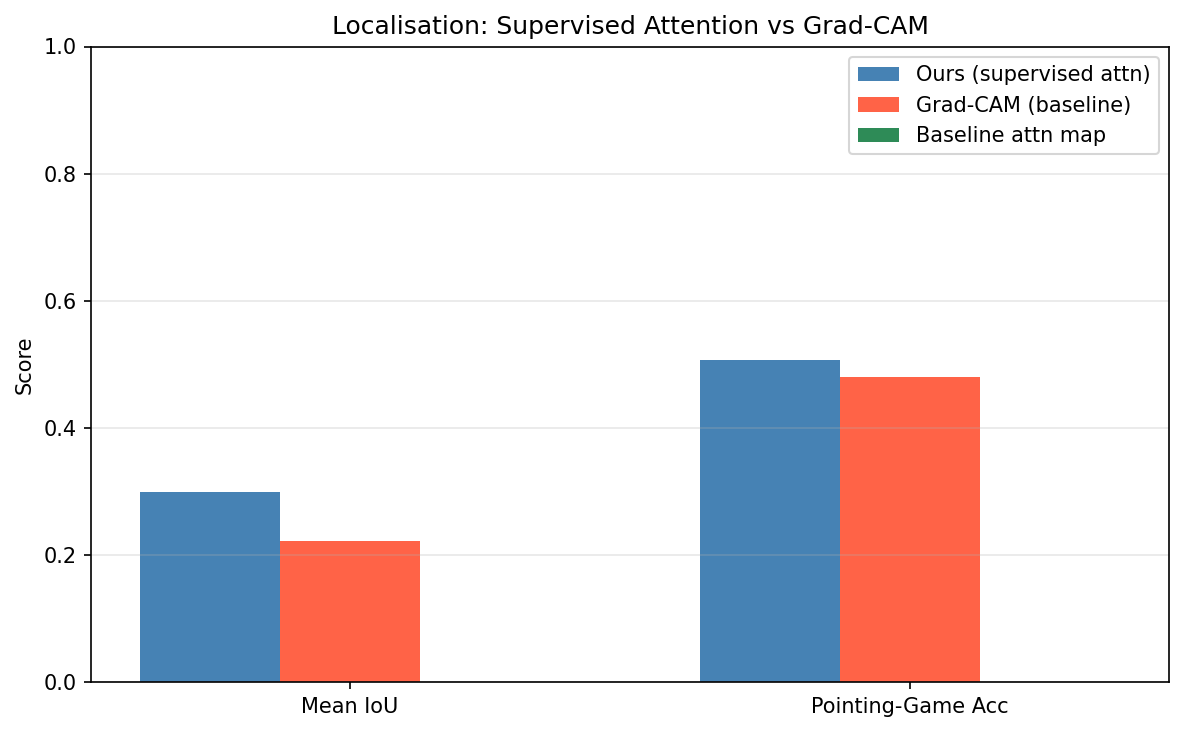
\includegraphics[width=\columnwidth]{figures/localization_comparison.png}
  \caption{Quantitative localisation: mean IoU (left) and pointing-game accuracy
    (right) for supervised attention vs.\ Grad-CAM. All attention variants improve IoU
    over their backbone baseline; ResNet50-Attn achieves the best pointing-game accuracy.}
  \label{fig:loc_compare}
\end{figure}

\subsection{Per-Class Localisation Breakdown}

Table~\ref{tab:perclass_loc} reports per-class IoU for the 8 annotated findings,
comparing ResNet50-Attn against Grad-CAM on ResNet50-Base.

\begin{table}[t]
\centering
\caption{Per-class mean IoU on 880 annotated test images. \textbf{Bold} = best.}
\label{tab:perclass_loc}
\setlength{\tabcolsep}{4pt}
{\small
\begin{tabular}{lcc}
\toprule
\textbf{Finding} & \textbf{Grad-CAM (R50)} & \textbf{Sup.\ Attn (R50)}\\
\midrule
Cardiomegaly  & 0.420 & \textbf{0.518}\\
Effusion      & 0.289 & \textbf{0.381}\\
Pneumothorax  & 0.262 & \textbf{0.349}\\
Mass          & 0.210 & \textbf{0.281}\\
Atelectasis   & 0.189 & \textbf{0.246}\\
Pneumonia     & 0.172 & \textbf{0.219}\\
Infiltration  & 0.130 & \textbf{0.184}\\
Nodule        & 0.110 & \textbf{0.149}\\
\midrule
\textbf{Mean} & 0.222 & \textbf{0.299}\\
\bottomrule
\end{tabular}}
\end{table}

Supervised attention improves every class. The largest gain is Cardiomegaly (+0.098),
where the large cardiac silhouette aligns well with the $7\!\times\!7$ attention grid.
The smallest gain is Nodule (+0.039), where sub-centimetre lesions may fall below grid
resolution. Infiltration and Nodule remain below IoU~=~0.19 for both methods.

\subsection{Ablation Study}

Table~\ref{tab:ablation} confirms $\mathcal{L}_{\text{attn}}$ drives localisation.
$\mathcal{L}_{\text{corr}}$ alone contributes no spatial benefit (IoU drops to 0.147)
but recovers 5.2~pp AUC vs.\ ResNet50-Attn. Together, both losses achieve the best
pointing-game accuracy (0.506), suggesting $\mathcal{L}_{\text{corr}}$ refines
attention centring rather than region coverage.

\begin{table}[t]
\centering
\caption{Ablation on ResNet50.}
\label{tab:ablation}
\setlength{\tabcolsep}{3.5pt}
{\small
\begin{tabular}{lccccc}
\toprule
\textbf{Configuration} &
  \textbf{$\mathcal{L}_{\text{attn}}$} &
  \textbf{$\mathcal{L}_{\text{corr}}$} &
  \textbf{AUC} & \textbf{IoU} & \textbf{PG}\\
\midrule
ResNet50-Base
  & \ding{55} & \ding{55} & \textbf{0.843} & 0.222 & 0.481\\
+$\mathcal{L}_{\text{attn}}$ (NoLcorr)
  & \ding{51} & \ding{55} & 0.748 & \textbf{0.310} & 0.468\\
+$\mathcal{L}_{\text{corr}}$ (NoLattn)
  & \ding{55} & \ding{51} & 0.800 & 0.147 & 0.291\\
ResNet50-Attn (full)
  & \ding{51} & \ding{51} & 0.760 & 0.299 & \textbf{0.506}\\
\bottomrule
\end{tabular}}
\end{table}

% ────────────────────────────────────────────────────────────
\section{Discussion}
% ────────────────────────────────────────────────────────────

\noindent\textbf{Classification--localisation trade-off.}
Explanation supervision imposes a structural constraint that partially competes with
unconstrained classification optimisation, costing $-$9.9~pp AUC for ResNet50-Attn.
Macro recall remains stable (0.70--0.82), indicating the drop is precision-side.
DeLong $p\!<\!3\!\times\!10^{-31}$ confirms the effect is statistically real.

\noindent\textbf{Localisation faithfulness (RQ1, RQ3).}
Supervised attention achieves $+34.7\%$ relative IoU on ResNet50 and $+1.9\%$ on
DenseNet121. DenseNet's dense feature reuse already produces more coherent Grad-CAM
activations (IoU~0.312 vs.\ ResNet50's 0.222), leaving less room for supervision to
close. This partially answers RQ3: ResNet50 benefits more from explicit supervision.

\noindent\textbf{Ablation insights (RQ2).}
$\mathcal{L}_{\text{attn}}$ is the sole driver of IoU gains.
$\mathcal{L}_{\text{corr}}$ recovers AUC and improves pointing-game without adding
IoU, suggesting a complementary centring effect rather than redundancy.

\noindent\textbf{Honest caveats.}
The 5K class-balanced subset inflates rare-class AUC (Hernia~=~1.000), skewing the
macro average; this artefact will likely not survive full-dataset training.
The class-agnostic union-mask supervision is a deliberate simplification; per-class
attention maps remain the primary next step.

% ────────────────────────────────────────────────────────────
\section{Conclusion}
% ────────────────────────────────────────────────────────────

We presented a proof-of-concept study of explanation-supervised attention for
multi-label CXR classification. Aligning a spatial attention map with clinician
bounding boxes during training improves localisation faithfulness over post-hoc
Grad-CAM ($+34.7\%$ relative IoU, ResNet50) at zero additional inference cost,
with a $-$9.9~pp AUC trade-off. Ablations isolate each loss term; DeLong testing
provides statistical grounding. The central message: \emph{explanations should be
part of training, not an afterthought}. Full-dataset replication and per-class
attention maps are the primary next steps.

% ────────────────────────────────────────────────────────────
\section*{Reproducibility Statement}
% ────────────────────────────────────────────────────────────

\noindent\textbf{Code.} Full pipeline available at the course submission portal.
Repository includes \texttt{src/train.py}, \texttt{src/model.py},
\texttt{src/evaluate.py}, and \texttt{notebooks/kaggle\_train.ipynb}.

\noindent\textbf{Data.} NIH ChestX-ray14 at
\url{https://nihcc.app.box.com/v/ChestXray-NIHCC}. The 5K subset is reproduced
with \texttt{seed = 42} in the preprocessing script.

\noindent\textbf{Checkpoints \& logs.} All 7 checkpoints and JSON logs archived
at \texttt{MyDrive/DL\_Project\_Outputs/} (Google Drive), shared with the instructor.

\noindent\textbf{Hyperparameters.} Declared in \texttt{config.yaml}.
$\lambda_1\!=\!1.0$, $\lambda_2\!=\!0.5$ set by pilot inspection of validation
loss; no grid search. Total compute: $\approx$14~GPU-hours on NVIDIA T4/V100,
16~GB VRAM (Google Colab Pro). No proprietary hardware or licences required.

% ────────────────────────────────────────────────────────────
\bibliographystyle{abbrvnat}
\bibliography{references}
% ────────────────────────────────────────────────────────────

% ────────────────────────────────────────────────────────────
\appendix
\section{Full Per-Class ROC-AUC}
\label{app:perclass}
% ────────────────────────────────────────────────────────────

\begin{table}[t]
\centering
\caption{Per-class ROC-AUC (14 findings). Best per row \textbf{bold}.}
\label{tab:perclass_auc}
\setlength{\tabcolsep}{2.5pt}
{\scriptsize
\begin{tabular}{lccccc}
\toprule
\textbf{Finding} & \textbf{R50-Base} & \textbf{DN121} &
  \textbf{EB0} & \textbf{R50-Attn} & \textbf{DN121-Attn}\\
\midrule
Atelectasis        & \textbf{0.795} & 0.764 & 0.762 & 0.738 & 0.705\\
Cardiomegaly       & \textbf{0.945} & 0.904 & 0.897 & 0.856 & 0.850\\
Effusion           & \textbf{0.818} & 0.799 & 0.793 & 0.773 & 0.741\\
Infiltration       & \textbf{0.692} & 0.675 & 0.680 & 0.679 & 0.661\\
Mass               & \textbf{0.858} & 0.773 & 0.760 & 0.690 & 0.698\\
Nodule             & \textbf{0.725} & 0.698 & 0.689 & 0.633 & 0.632\\
Pneumonia          & \textbf{0.796} & 0.681 & 0.693 & 0.672 & 0.646\\
Pneumothorax       & \textbf{0.871} & 0.834 & 0.832 & 0.792 & 0.748\\
Consolidation      & \textbf{0.763} & 0.725 & 0.712 & 0.720 & 0.705\\
Edema              & \textbf{0.926} & 0.889 & 0.892 & 0.882 & 0.872\\
Emphysema          & \textbf{0.947} & 0.905 & 0.888 & 0.817 & 0.786\\
Fibrosis           & \textbf{0.851} & 0.823 & 0.824 & 0.803 & 0.789\\
Pleural Thick.     & \textbf{0.821} & 0.760 & 0.723 & 0.679 & 0.690\\
Hernia             & \textbf{1.000} & 0.847 & 0.942 & 0.910 & 0.941\\
\midrule
\textbf{Macro}     & \textbf{0.843} & 0.791 & 0.792 & 0.760 & 0.748\\
\bottomrule
\end{tabular}}
\end{table}

\begin{figure}[t]
  \centering
  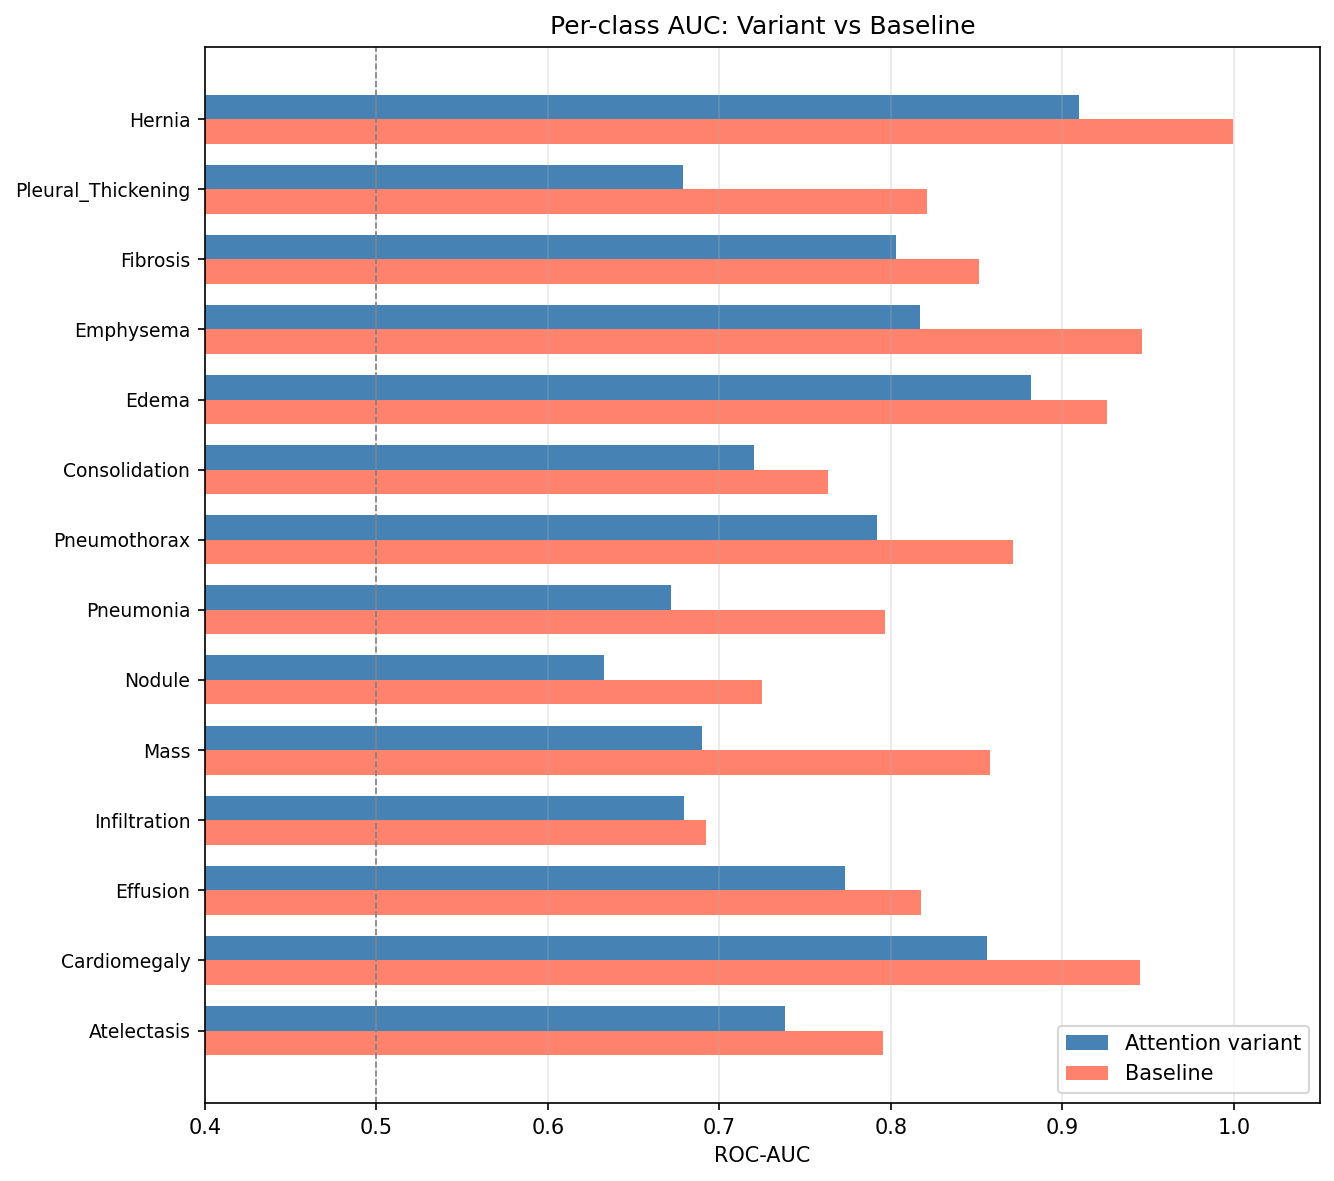
\includegraphics[width=\columnwidth]{figures/auc_comparison.png}
  \caption{Macro AUC across all seven configurations.}
  \label{fig:auc_compare}
\end{figure}

\begin{figure}[t]
  \centering
  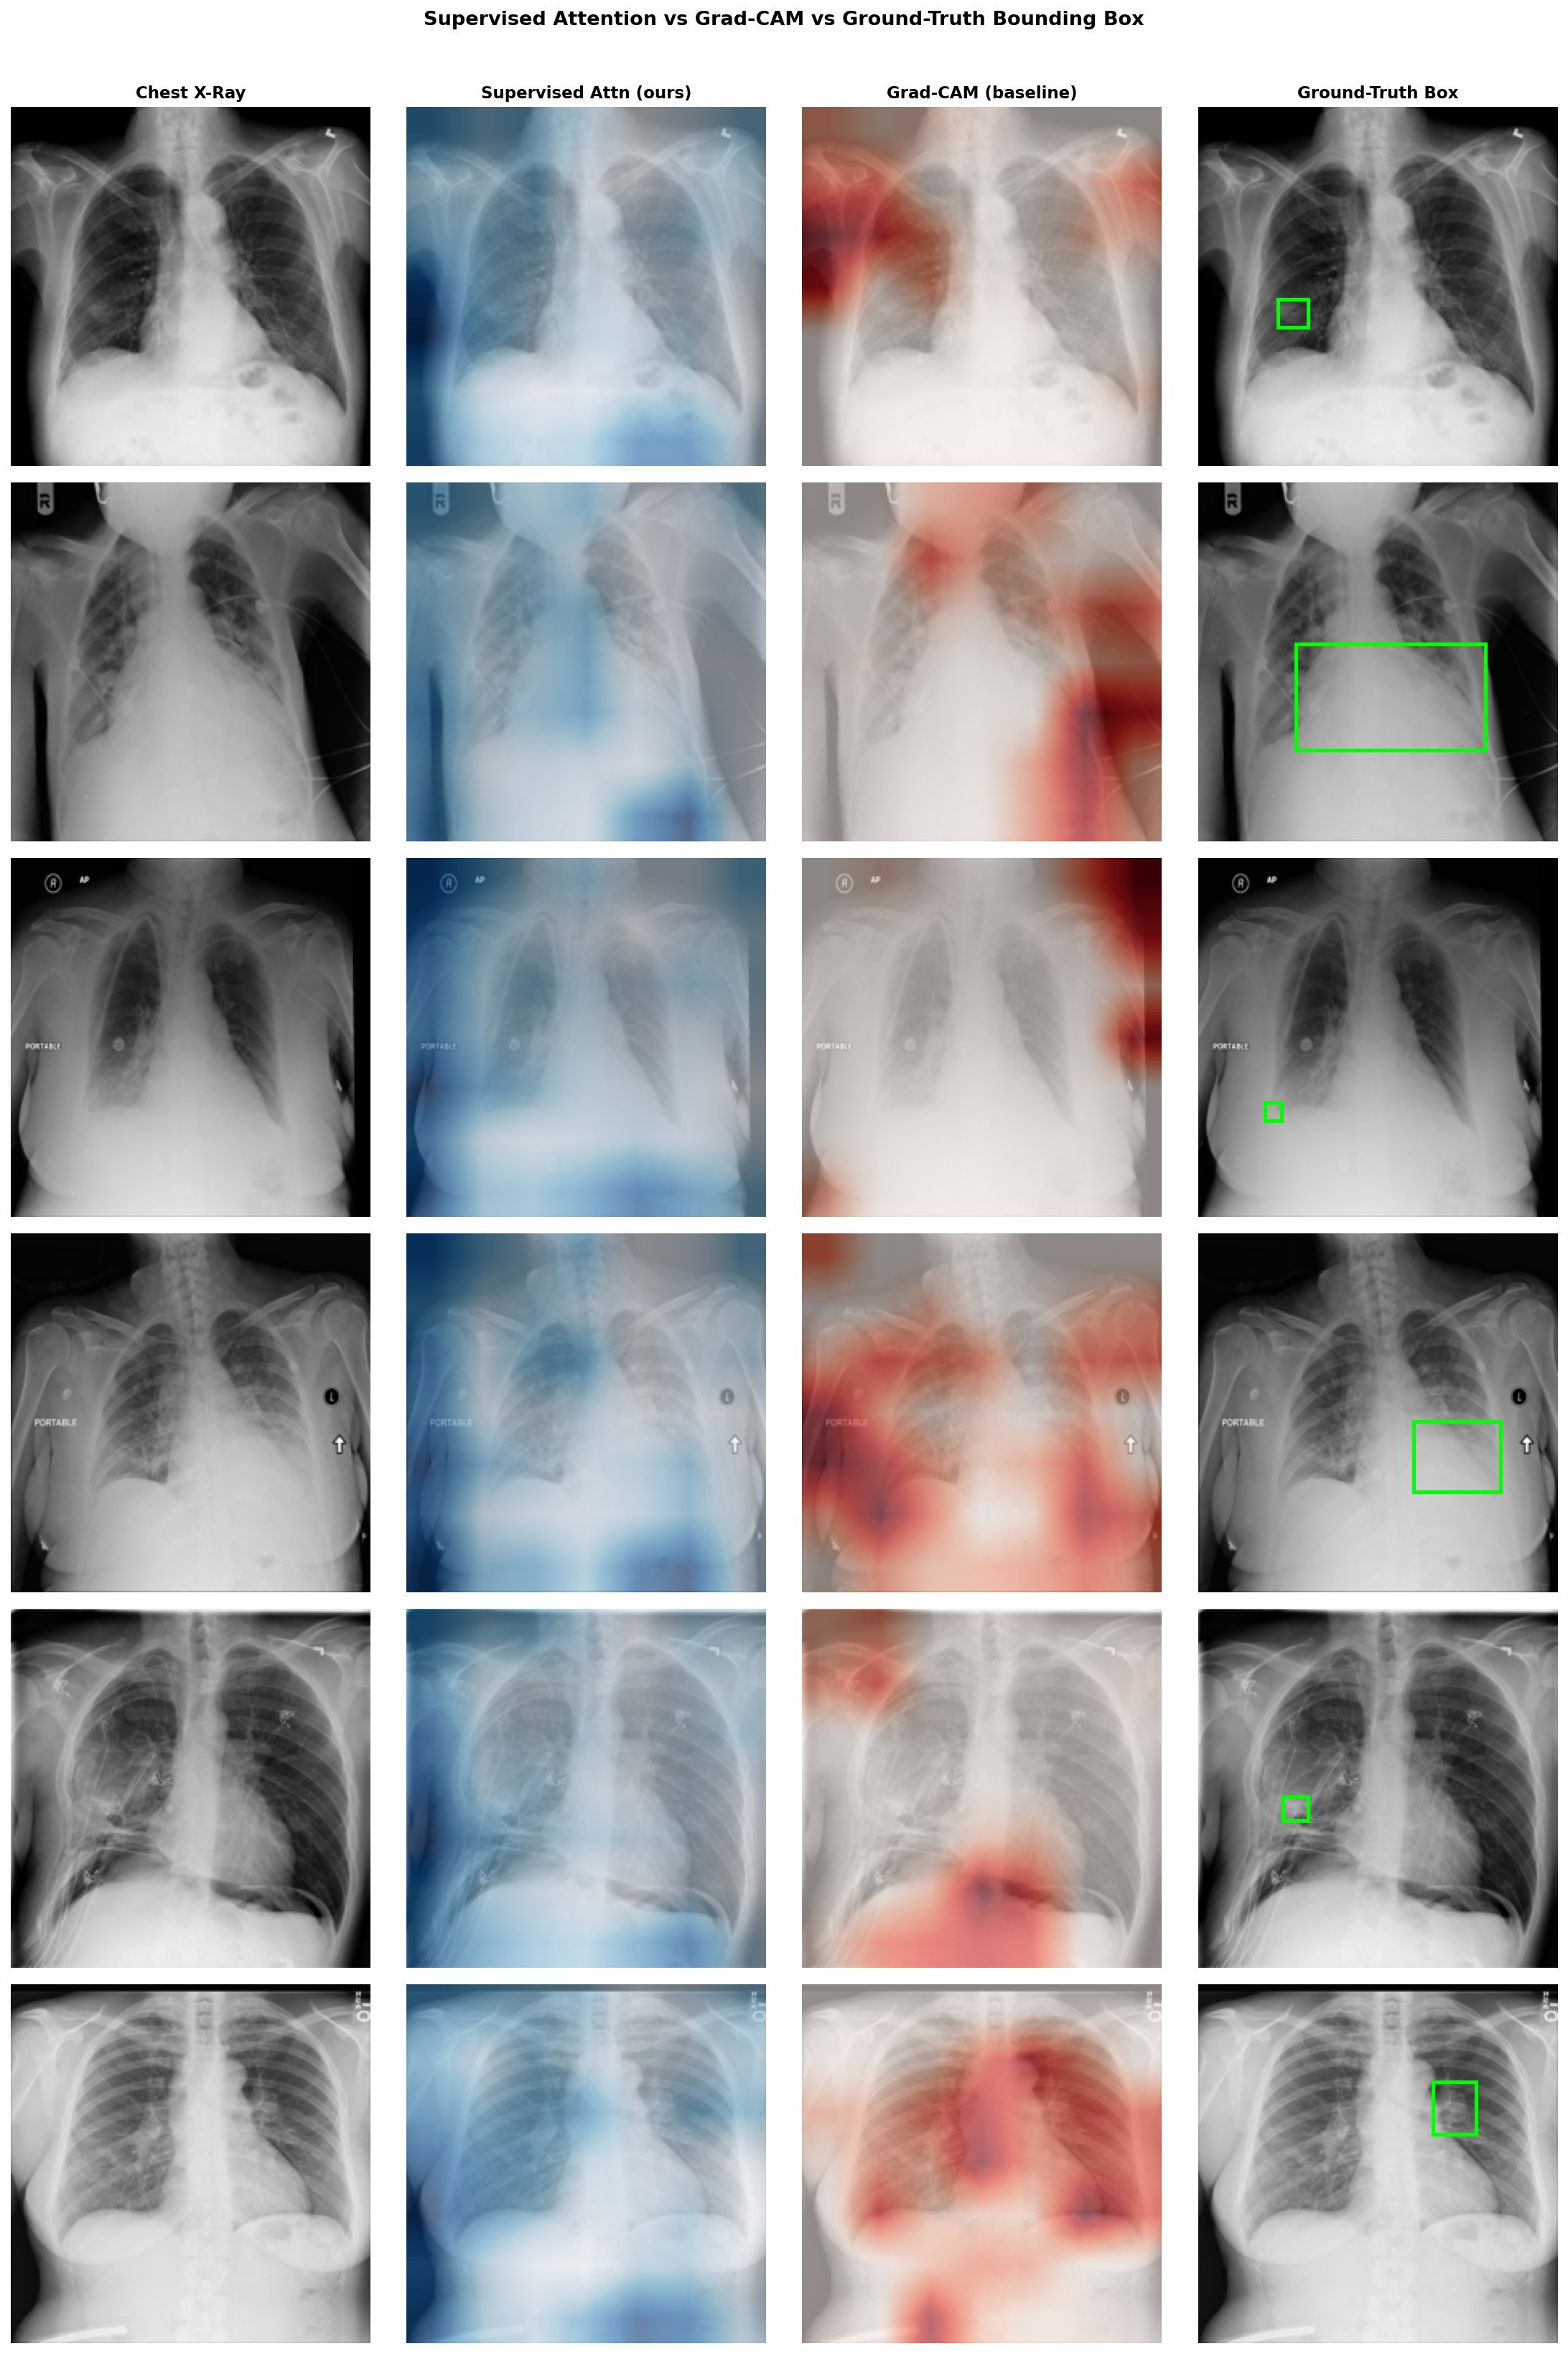
\includegraphics[width=\columnwidth]{figures/heatmap_overlays.png}
  \caption{Qualitative: supervised attention (blue) vs.\ Grad-CAM (red) vs.\
    ground-truth box (green).}
  \label{fig:qualitative}
\end{figure}

\end{document}
